\section{Laplace approximation}
One approach to approximating the posterior parameter probability, is to use a second degree polynomial to approximate the aggregate loss function $\mathcal L(\theta)\propto - \ln p(\mathcal{D} \vert\theta) - \ln p(\theta)$. In practice, this is done by finding a Maximum Aposteriori (MAP) estimate $\theta^\ast$, that  minimizes $\mathcal L(\theta)$. The Laplace approximation is then the normal distribution with mean $\theta^\ast$ and the same covariance matrix $\Sigma_0$ as $p(\theta \vert \mathcal D)$ has locally around $ \theta^\ast$.

Let $B_0$ be the hessian of the loss, with respect to the parameters:
$B(\theta) \coloneq - \mathbf{H}_{\theta}[\mathcal{L(\theta)}].$
Then if $\Sigma_{\theta^\ast} = B^{-1}(\theta^\ast)$ is positive semi-definite, we can define a Gaussian distribution $q(\theta) \sim \mathcal N( \theta^\ast, \Sigma_{\theta^\ast})$ which has the property that $\left. \mathbf{H}_{\theta}[\ln q(\theta)]\right\vert_{\theta^\ast} =\Sigma_{\theta^\ast}$, meaning that the log of the approximate distribution $q(\theta)$ has the same Hessian as the log of the true posterior distribution $p(\theta\vert\mathcal{D})$.

For smaller models, and models where the posterior distribution is guaranteed locally approximately Gaussian, this can be a good solution. However, as the dimensionality of the parameter space increases, the probability that the posterior distribution is non-Gaussian along at least one of the axes increases, leading to low-likelihood parameter samples.

The Laplace approximation class used in this paper is built to allow for subspace sampling. That is, if $A$ is an eigenvector decomposition of $\Sigma_{\theta^\ast}$ such that $A^\top A = \Sigma_{\theta^\ast}$ and $\varepsilon \sim \mathcal N(\bm 0,\bm I_d)$ then we also have that $\theta = \theta^\ast +A \varepsilon$. 
If we then let $A_k$ be the first $k$ columns of $A$, and sample $\varepsilon_k \sim \mathcal N(\bm 0,\bm I_k)$, we can reduce the space that $\theta$ is sampled from, by setting $\theta_k = \theta^\ast +A \varepsilon_k$. 

In figure \ref{fig:UFA_laplace_prob}, the posterior density of the function approximator, sliced along the direction of the eigenvectors belonging to the two dominant eigenvalues of the covariance matrix, is displayed along with its Laplace approximation. As can be seen in this example, the Laplace approximation has relatively much support for parameter values that gives rise to high loss. This is problematic, since parameter samples from these areas will result in wildly wrong prediction functions, which in turn means too wide prediction bands.

\begin{figure}[h]
    \centering
    \subfloat[First eigendirection of the function approximator posterior]{
        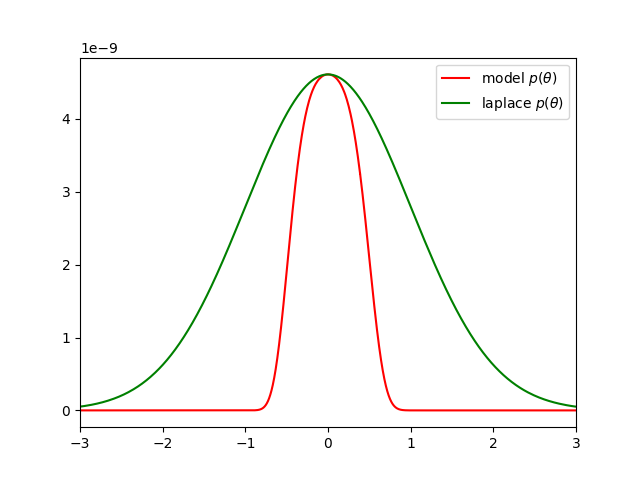
\includegraphics[width=.31\linewidth]{report/figures/UFA_laplace_prob.png}
        \label{fig:UFA_laplace_prob}
    }
    \hfill
    \subfloat[Full rank Laplace approximation of the function approximator]{
        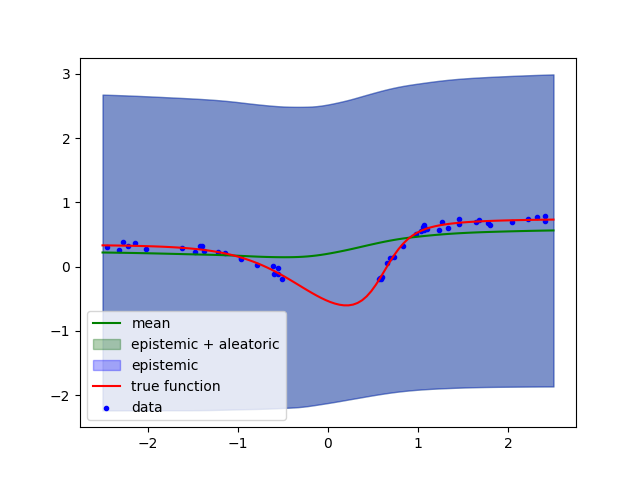
\includegraphics[width=.31\linewidth]{report/figures/laplace_approximation_fullrank.png}
        \label{fig:laplace_approximation_fullrank}
    }
    \hfill
    \subfloat[Rank-2 Laplace approximation of the function approximator]{
        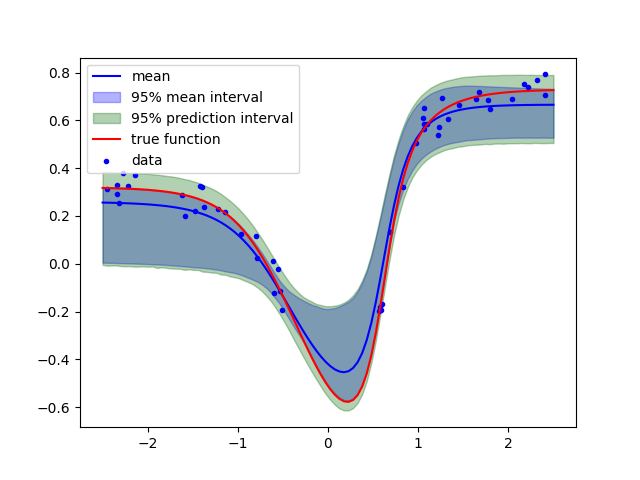
\includegraphics[width=.31\linewidth]{report/figures/laplace_approximation_subspace_rank2.png}
        \label{fig:laplace_approximation_subspace_rank1}
    }
    \hfill
    \caption{Laplace approximations}
    \label{fig:laplace_approximations}
\end{figure}

Similarly for the universal function estimator. When using the full Laplace approximation, we see some terrible parameter sampling with a mean that does not follow the true mean, and extremely wide prediction bands as seen in figure \ref{fig:laplace_approximation_fullrank}. If samples are only taken from the most important eigendirections of the covariance matrix, the results improve drastically as seen in figure \ref{fig:laplace_approximation_subspace_rank1}. We do however still see much overestimation of uncertainty due to highly improbable parameter samples as seen in figure \ref{fig:UFA_laplace_prob}. 